\documentclass[10pt,twocolumn]{article}
%%%%%%%%%%%%%%%%%%%%%%%%%
%			AZ' STANDARD NEWCOMMANDS
%%%%%%%%%%%%%%%%%%%%%%%%%
\usepackage[english]{babel}
\usepackage[T1]{fontenc}
\usepackage{cite, url,color} % Citation numbers being automatically sorted and properly "compressed/ranged".
%\usepackage{pgfplots}
\usepackage{graphics,amsfonts}
\usepackage[pdftex]{graphicx}
\usepackage[cmex10]{amsmath}
% Also, note that the amsmath package sets \interdisplaylinepenalty to 10000
% thus preventing page breaks from occurring within multiline equations. Use:
\interdisplaylinepenalty=2500
% after loading amsmath to restore such page breaks as IEEEtran.cls normally does.
\usepackage[utf8]{inputenc}
% Useful for dispalying quotations
\usepackage{csquotes}
% Compact lists
\usepackage{enumitem}

\usepackage{array}
% http://www.ctan.org/tex-archive/macros/latex/required/tools/
\usepackage{mdwmath}
\usepackage{mdwtab}
%mdwtab.sty	-- A complete ground-up rewrite of LaTeX's `tabular' and  `array' environments.  Has lots of advantages over
%		   the standard version, and over the version in `array.sty'.
% *** SUBFIGURE PACKAGES ***
\usepackage[tight,footnotesize]{subfigure}

\usepackage[top=1.5cm, bottom=2cm, right=1.6cm,left=1.6cm]{geometry}
\usepackage{indentfirst}

\usepackage{times}
% make sections titles smaller to save space
\usepackage{sectsty}
\sectionfont{\large}
% enable the use of 'compactitem', a smaller 'itemize'
\usepackage{paralist}

\setlength\parindent{0pt}
\linespread{1}

\def\C#1{\mathcal{#1}}

\renewcommand{\phi}{\varphi}
% OPERATORS
\newcommand{\floor}[1]{{\left\lfloor #1\right\rfloor}}
\newcommand{\ceil}[1]{{\left\lceil #1\right\rceil}}
\newcommand{\E}[1]{\mathop{\rm E}\nolimits\left[#1\right]} % Expectation
\newcommand{\pr}[1]{\Pr\left[ #1 \right]}
\renewcommand{\P}[1]{\mathrm{P}\left[ #1 \right]}

\newcommand{\mbb}{\mathbb}
\newcommand{\mee}{\mathrm{e}}
\newcommand{\mrr}{\mathrm}
\newcommand{\m}{\mathrm{m}}
\newcommand{\mmin}[1]{{\min\left\{#1\right\}}}
\newcommand{\mmax}[1]{{\max\left\{#1\right\}}}
\newcommand{\id}[1]{\mathbf{1}\(#1\)} % Unit function
\newcommand{\Heav}[1]{H\left(#1\right)} % Heaviside function
\newcommand{\eps}{\varepsilon}
\newcommand{\rect}[1]{\mathrm{rect}\!\left(#1\right)}
\newcommand{\sinc}[1]{\mathrm{sinc}\!\left(#1\right)}
\newcommand{\bin}[2]{{\left(\begin{array}{c}#1\\#2\end{array}\right)}}

\newcommand{\me}[2]{\left[ {#1} \right]_{(#2)}} % Submatrix \me{P}{i,j} produces [P]_{i,j} and denotes the element in the i-th row and j-th column of P
\newcommand{\vv}[1]{\left[ {#1} \right]} % Submatrix \vv{a,b,c} produces [a,b,c]

\newcommand{\Set}[1]{{\C #1}}
\newcommand{\Setd}[2]{\Set{#1}=\left\{#2\right\}}  % Set definition: \Set{S}{0,1,2} produces S={01,2,} where S is in mathcal

\newcommand{\mat}[1]{{\hbox{\textbf{#1}}}}
\newcommand{\ei}[1]{{\mat{e}_{#1}}}   % all zero vector except in the $#1$-th element which is one
\newcommand{\ind}[1]{\mathbf{\chi}\left\{#1\right\}} % Indicator function \ind{A}=1 if A is true, \ind{A}=0 otherwise.

% FORMATTING
\newcommand{\ie}{i.e.,\,}
\newcommand{\eg}{e.g.,\,}
\newcommand{\columnbreak}{\vfill\eject} % Column break

% REFERENCES
\newcommand{\Fig}[1]{Fig.~\ref{#1}}
\newcommand{\eq}[1]{(\ref{#1})}
\newcommand{\Tab}[1]{Tab.~\ref{#1}}
\newcommand{\Sec}[1]{Sec.~\ref{#1}}

\begin{document}
\title{HIPSTER, the alternative file transfer protocol}
\author{}
\date{}
\maketitle

\section{Introduction}
In this paper we will describe the HIPSTER protocol, a file transfer protocol designed to work on top of the UDP transport layer. The aim of the protocol is to minimize transfer time over an unreliable Transport Channel (TC), which introduces delay and drops packet according to a certain model. In the first section, the protocol will be described. Then, we will show the results of some tests for the TC, demonstrating that it works as specified by the model. In the last section test results will be presented and we will show that the system reaches low transfer times.

\section{Protocol description}
\begin{figure}[htp]
	\centering
	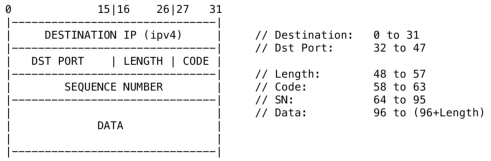
\includegraphics[width=0.95\columnwidth]{tex/images/packet_structure.pdf}
	\caption{HIPSTER packet structure}
	\label{fig:header}
\end{figure}

The packet structure has been designed in order to add the minimum overhead,
while providing all the functionality needed by the protocol.

Destination IP and port are needed for packet forwarding within the channel
and by the receiver for replying to the sender. The first two fields are the
same within different groups. Moreover the size of the payload was included to 
ease the parsing of the packet at the receiving side. Finally \texttt{CODE} and
\texttt{SEQUENCE NUMBER} are used for signalling and error recovery.

The following values are used for the code:
\begin{compactitem}
\item 0 means a regular data packet
\item 1 carries an ACK, the sequence number received is the same as the packet
	being ACKed and no payload
\item 2 signals the end of transmission (ETX). It is issued by the sender and
	ACKed by the receiver
\end{compactitem}

Before the actual implementation a theoretical model of the protocol and the
channel was developed. Such model showed that the optimal packet length to
minimize the transfer time is around 1000 byte so this protocol uses fixed-size
packets whose payload length is 1000 byte.

The behaviour of the sender (DS) is depicted in Figure~\ref{fig:senderFlow}.
It is organized into two threads: ListenerThread which receives, decodes and
enqueues ACKs and SendThread that is in charge of sending all packets
successfully and performing some basic congestion control using the enqueued
ACKs.
\begin{figure}[htp]
	\centering
	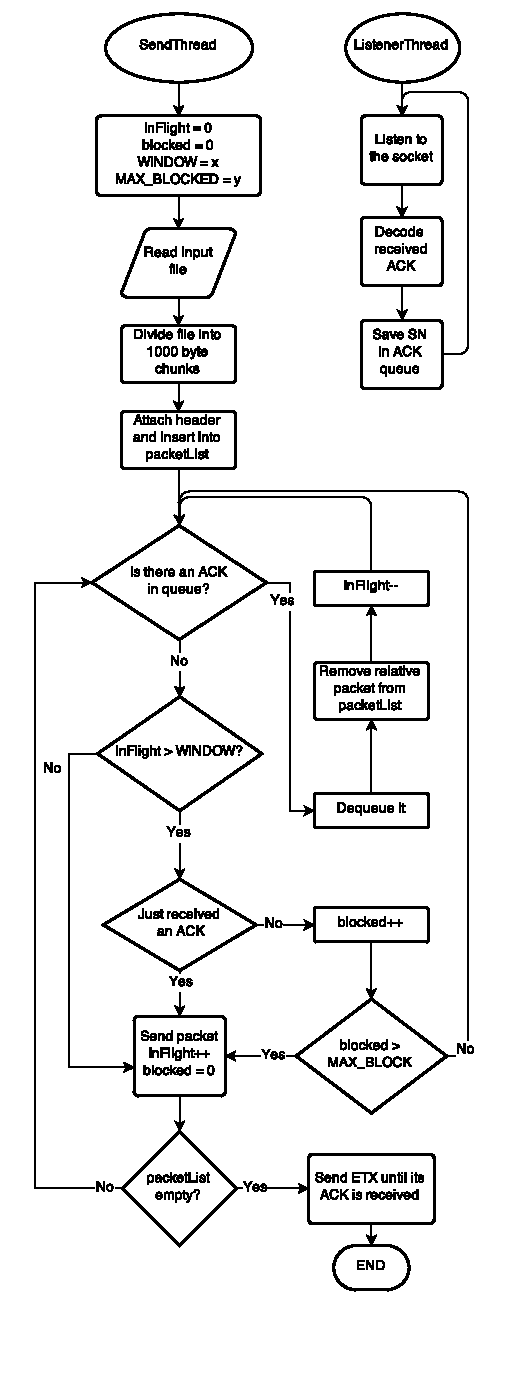
\includegraphics[height=0.75\textheight]{Documentation/Sender.pdf}
	\caption{HIPSTER protocol DS}
	\label{fig:senderFlow}
\end{figure}

Basically the \texttt{inFlight} counter in SendThread is increased every time
a packet is sent and decreased when an ACK is received. DS sends packets
continuously until \texttt{inFlight} has reached the maximum allowed window.
When the window is full the sender won't send packets continuously but will
send a packet every time an ACK is received. The \texttt{blocked} counter is
used to avoid deadlocks in case some ACKs are lost: it sets a maximum delay 
before a packet is sent regardless of the received ACK.
Every time an ACK is dequeued the corresponding packet is removed from the
list of packets. Only when the list is empty the transmission is considered
complete. At this time DS sends the ETX packet which signals to the receiver 
that the transmission is over. If the corresponding ACK is received the sender
will exit otherwhise if a $2.5s$ timer expires the ETX is sent again.

The Receiver is in charge of handling ACK transmission and the reordering of the received packets. The protocol assumes the random delays and drops introduced by the channel would make in-order delivery extremely slow, so the decision of shifting the burden of reordering on the receiver was made. The Receiver listens continuously for new packets. Once it receives a packet, it checks its CODE. If the CODE is DATA, the DR stores the packet in a list and sends an ACK to the Sender through the Channel. In the case the received packet contains an ETX (end of transmission) code, the Receiver acknowledges it, then proceeds to reorder the packets and finally writes the received file to disk. The ACKs crafted by the Receiver contain an empty payload in order to minimize the channel drop probability, and the sequence number refers to the single packet the Receiver intends to acknowledge, in order to inform the Sender that retransmission of that portion is not necessary.

\begin{figure}[h]
  \centering
  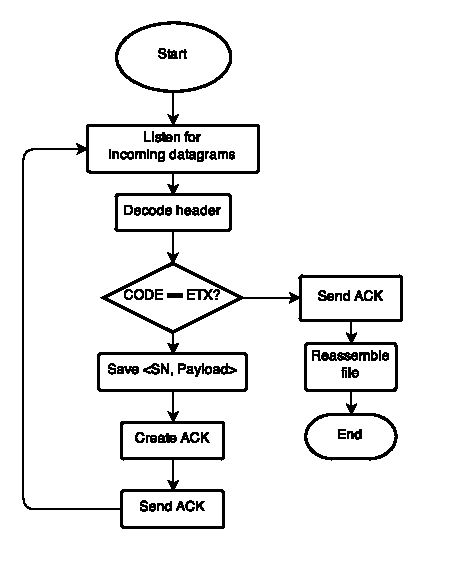
\includegraphics[width=0.75\columnwidth, keepaspectratio]{Documentation/Receiver.pdf}
  \caption{HIPSTER protocol DR}
  \label{fig:receiverFlowchart}
\end{figure}

\section{Transport Channel test results}
The Transport Channel (TC) module simulates a bad channel among the DS and DR. It drops received UDP packets of length $L$ with probability $P_{drop} = 1 - \exp(-L/1024)$ and forwards the remaining ones with a delay distribuited according to an expontial random variable with mean $1024/\ln(L)$ ms. \\
The TC was tested in loopback, by measuring the delay between the transmission of a packet by DS and its reception at DR and the ratio between sent and received packets. The payload of UDP packet used in this test is in the range from 12 byte (HIPSTER header length, thus the size of an ACK) to 1012 byte (actual size of HIPSTER packets). Each measurement was taken 10 times. The results are in figures~\ref{fig:pDrop} and~\ref{fig:delay}. The TC follows accurately the theoretical model, the few discrepancies are related to the Java random number generator and the finiteness of measurements. The distribution of the delays introduced by the TC in a transmission fits the required exponential RV according to the Kolmogorov-Smirnov test and the comparison of the cumulative distributive functions (CDF) of the two can be seen in figure~\ref{fig:CDF}.

%this third figure can be omitted
\begin{figure}[h!]
  \centering
  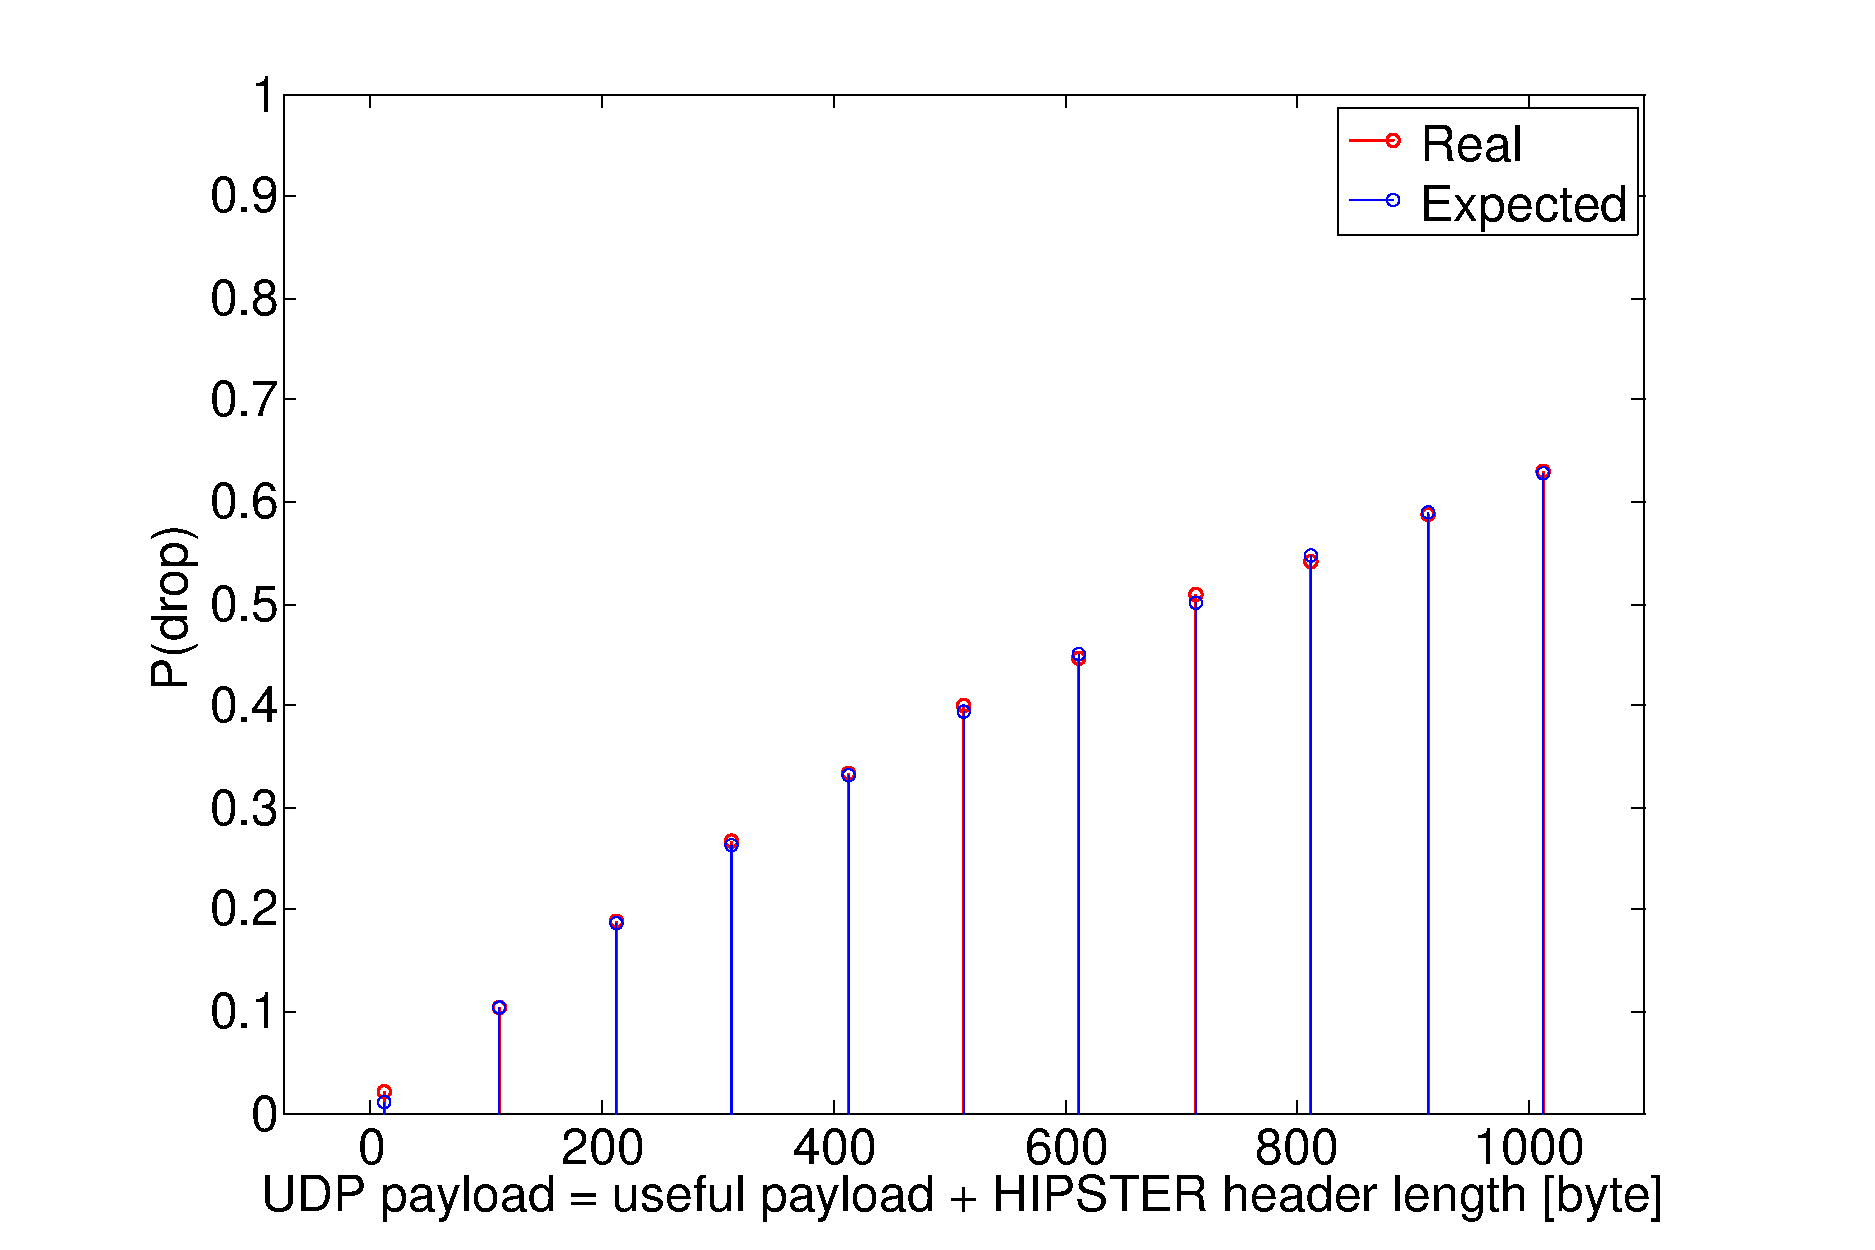
\includegraphics[width=0.95\columnwidth, keepaspectratio]{tex/images/pdrop.pdf}
  \caption{Dropping probability}
  \label{fig:pDrop}
\end{figure}

\begin{figure}[h!]
  \centering
  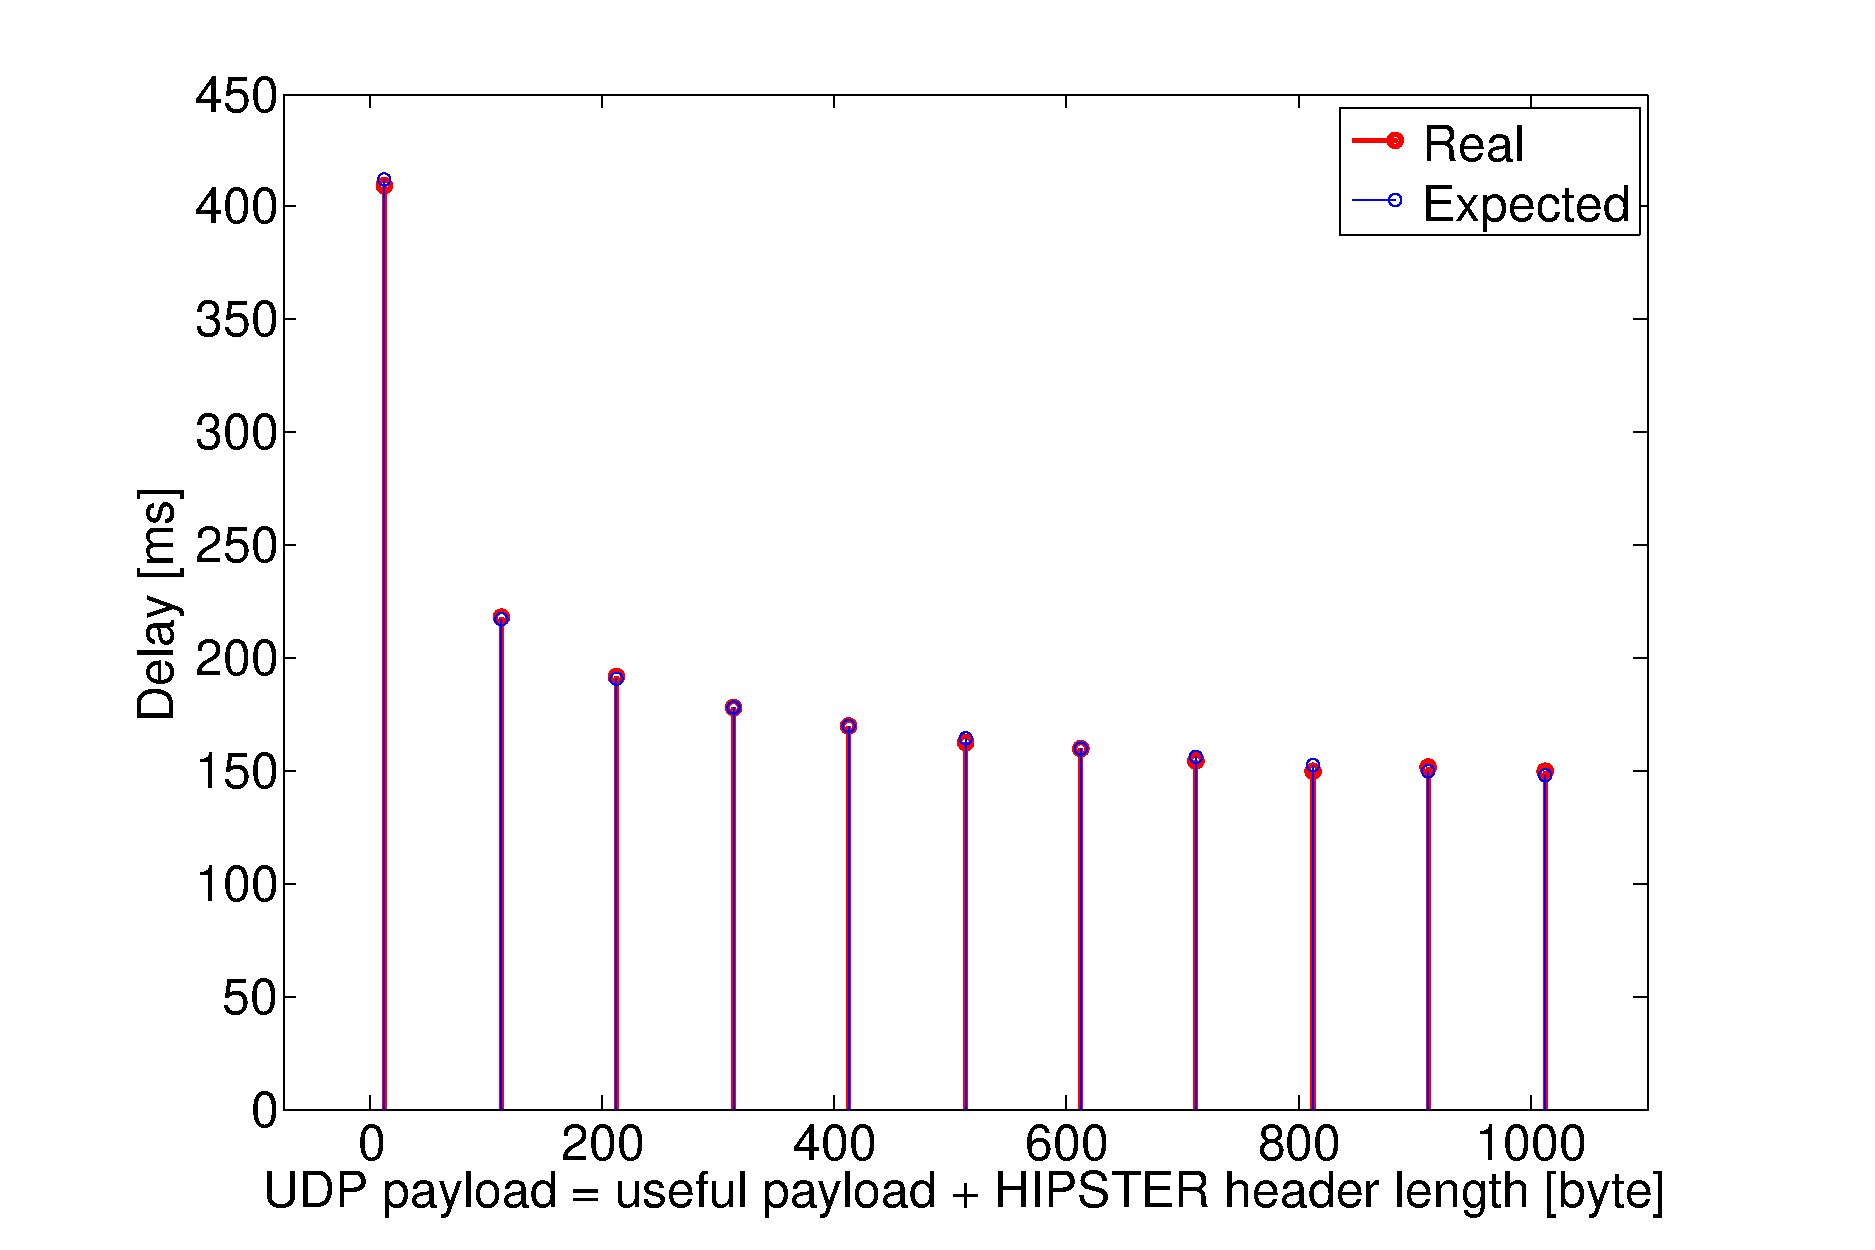
\includegraphics[width=0.95\columnwidth, keepaspectratio]{tex/images/delayChannel.pdf}
  \caption{Mean TC delay}
  \label{fig:delay}
\end{figure}

\begin{figure}[h!]
  \centering
  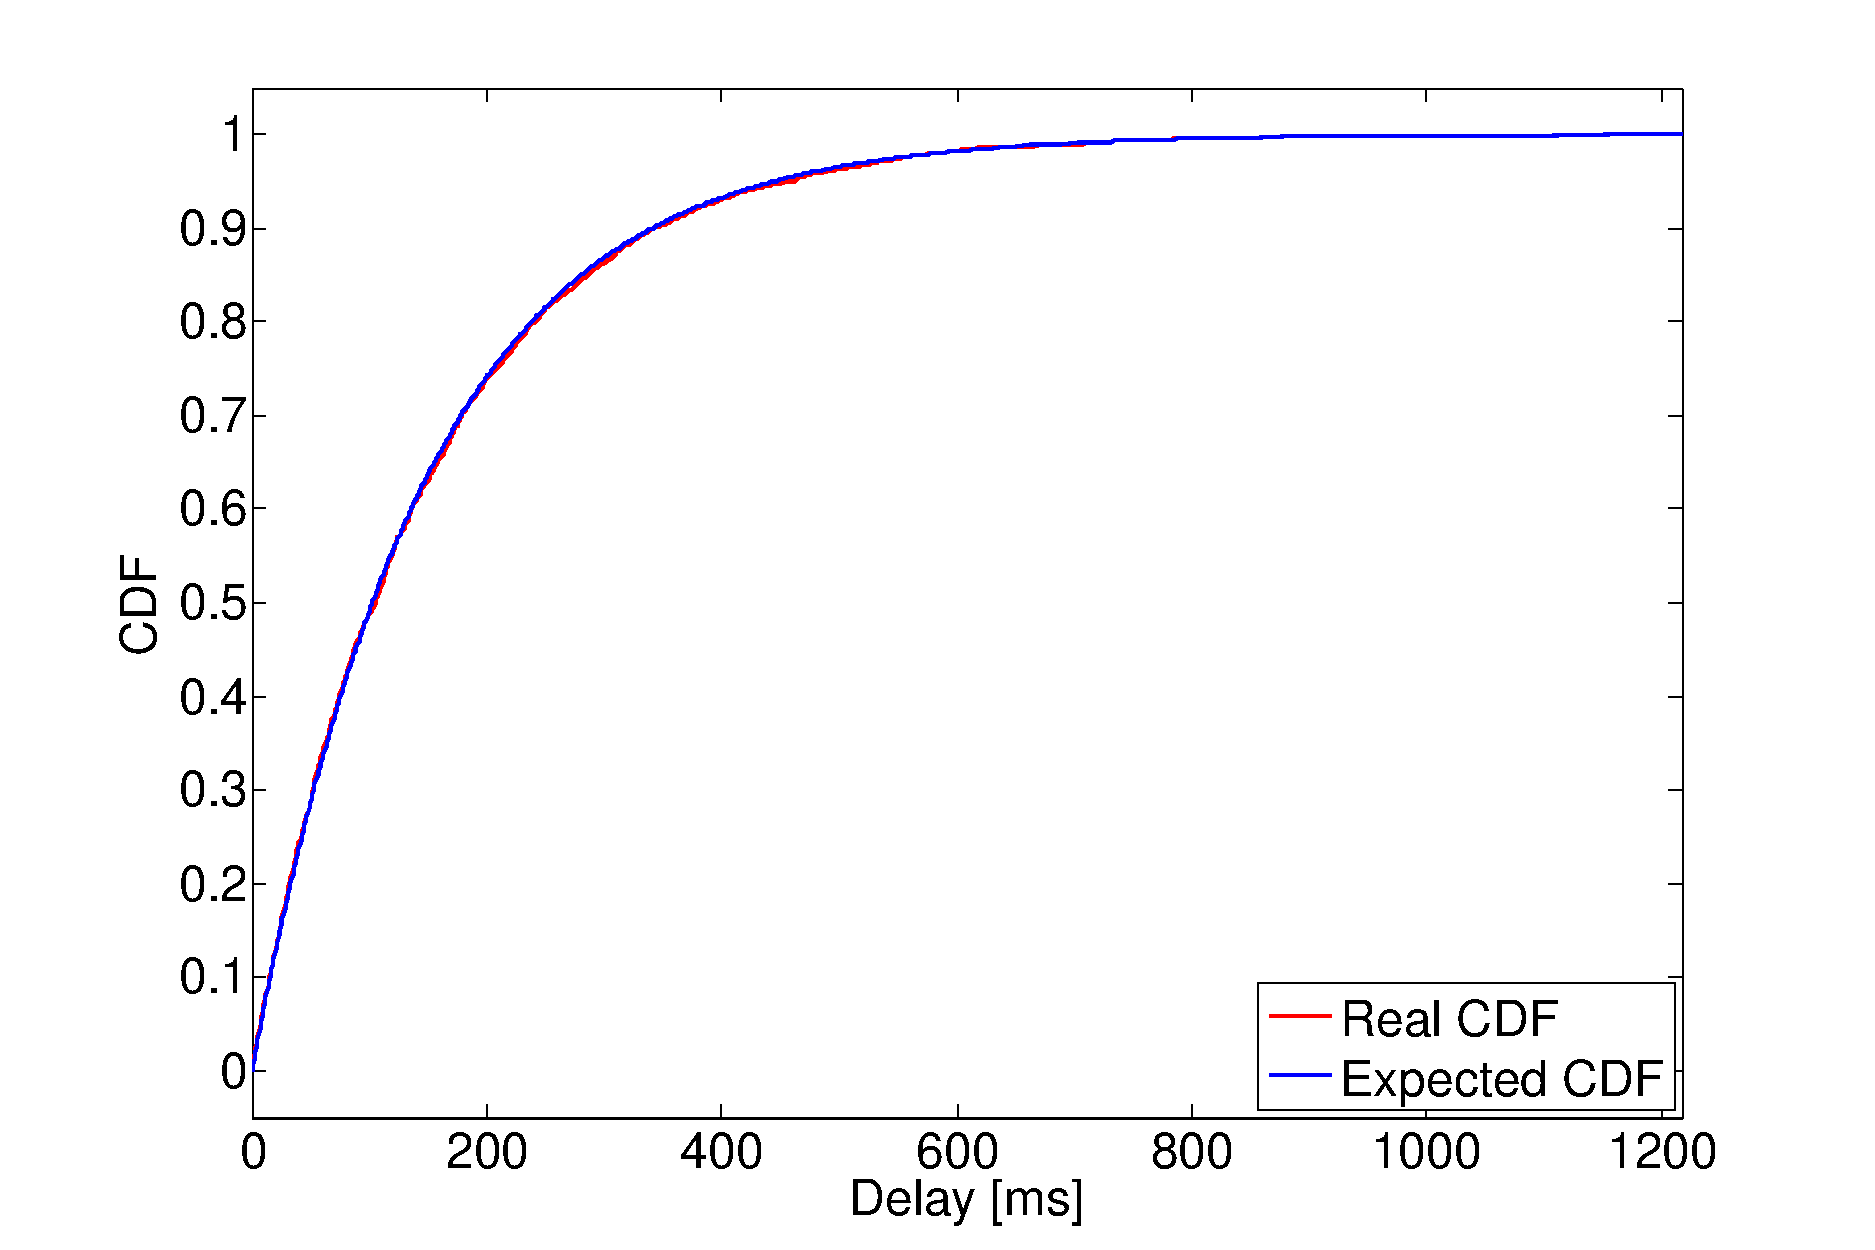
\includegraphics[width = 0.95\columnwidth, keepaspectratio]{tex/images/cdfChannel.pdf}
  \caption{CDF of delays introduced by TC, $L_{UDP} = 1012$ byte}
  \label{fig:CDF}
\end{figure}

\section{HIPSTER protocol test results}
The transfer rate for files with different sizes was analyzed. The
table~\ref{table:ourChannel} summarizes the mean over five runs for the transfer time and speed for
\texttt{localhost}, while the table~\ref{table:anotherChannel} reports the
results of the same tests with another channel, borrowed from a different group. \textit{Mean time} is the time from the beginning of the transmission at the Sender to the reception of the ACK for the ETX packet, while \textit{mean goodput} is file size over \textit{mean time}.
\begin{table}[h]
\centering
\begin{tabular}{|c|c|c|}
	Size (MB) & Mean time (s) & Mean goodput (MB/s)\\ \hline
  500       & 64.92    & 8.07  \\
  200       & 23.86    & 8.78  \\
	100       & 13.48    & 7.78  \\
	50        & 7.83     & 6.7 \\
	10        & 2.57     & 4.07 \\
	5         & 1.55     & 3.39  \\
	1         & 0.67     & 1.56  \\
\end{tabular}
\label{table:ourChannel}
\end{table}

\begin{table}[h]
\centering
\begin{tabular}{|c|c|c|}
  Size (MB) & Mean time (s) & Mean goodput (MB/s)\\ \hline
  500       & 62.63    & 8.37  \\
  200       & 23.54    & 8.9  \\
  100       & 14.04    & 7.47  \\
  50        & 7.85     & 6.67 \\
  10        & 2.4      & 4.34 \\
  5         & 1.56     & 3.35 \\
  1         & 0.67     & 1.56 \\

\end{tabular}
\label{table:anotherChannel}
\end{table}

Tests in a Local Area Network yield similar results. The transfer rate over different ADSL and WiMax links has also been tested. In
this scenario the algorithm needed some tuning of the \texttt{MAX\_BLOCK}
constant due to excessive congestion. Such variable has to be adapted to
different networks. Bigger values (in the order of $10^5$) are better suited
for slow networks with longer RTTs. Smaller values instead (e.g.\ the default
128) are better suited to fast networks with RTT of about 1 ms. \\
The goodput at the Receiver over time is in figures~\ref{fig:goodput_200} and~\ref{fig:goodput_500}. They show the number of useful bit received every 500 ms, normalized to this sampling time, for a 200 MB file and 500 MB transmission. Both the figures show a common trend, with high goodput at the beginning which decreases once transmission is almost completed, because of retransmission mechanism and long delays for the ACKs in the TC. The sudden drops of the goodput, instead, signal that congestion control mechanism has kicked in.\\

\begin{figure}[h]
  \centering
  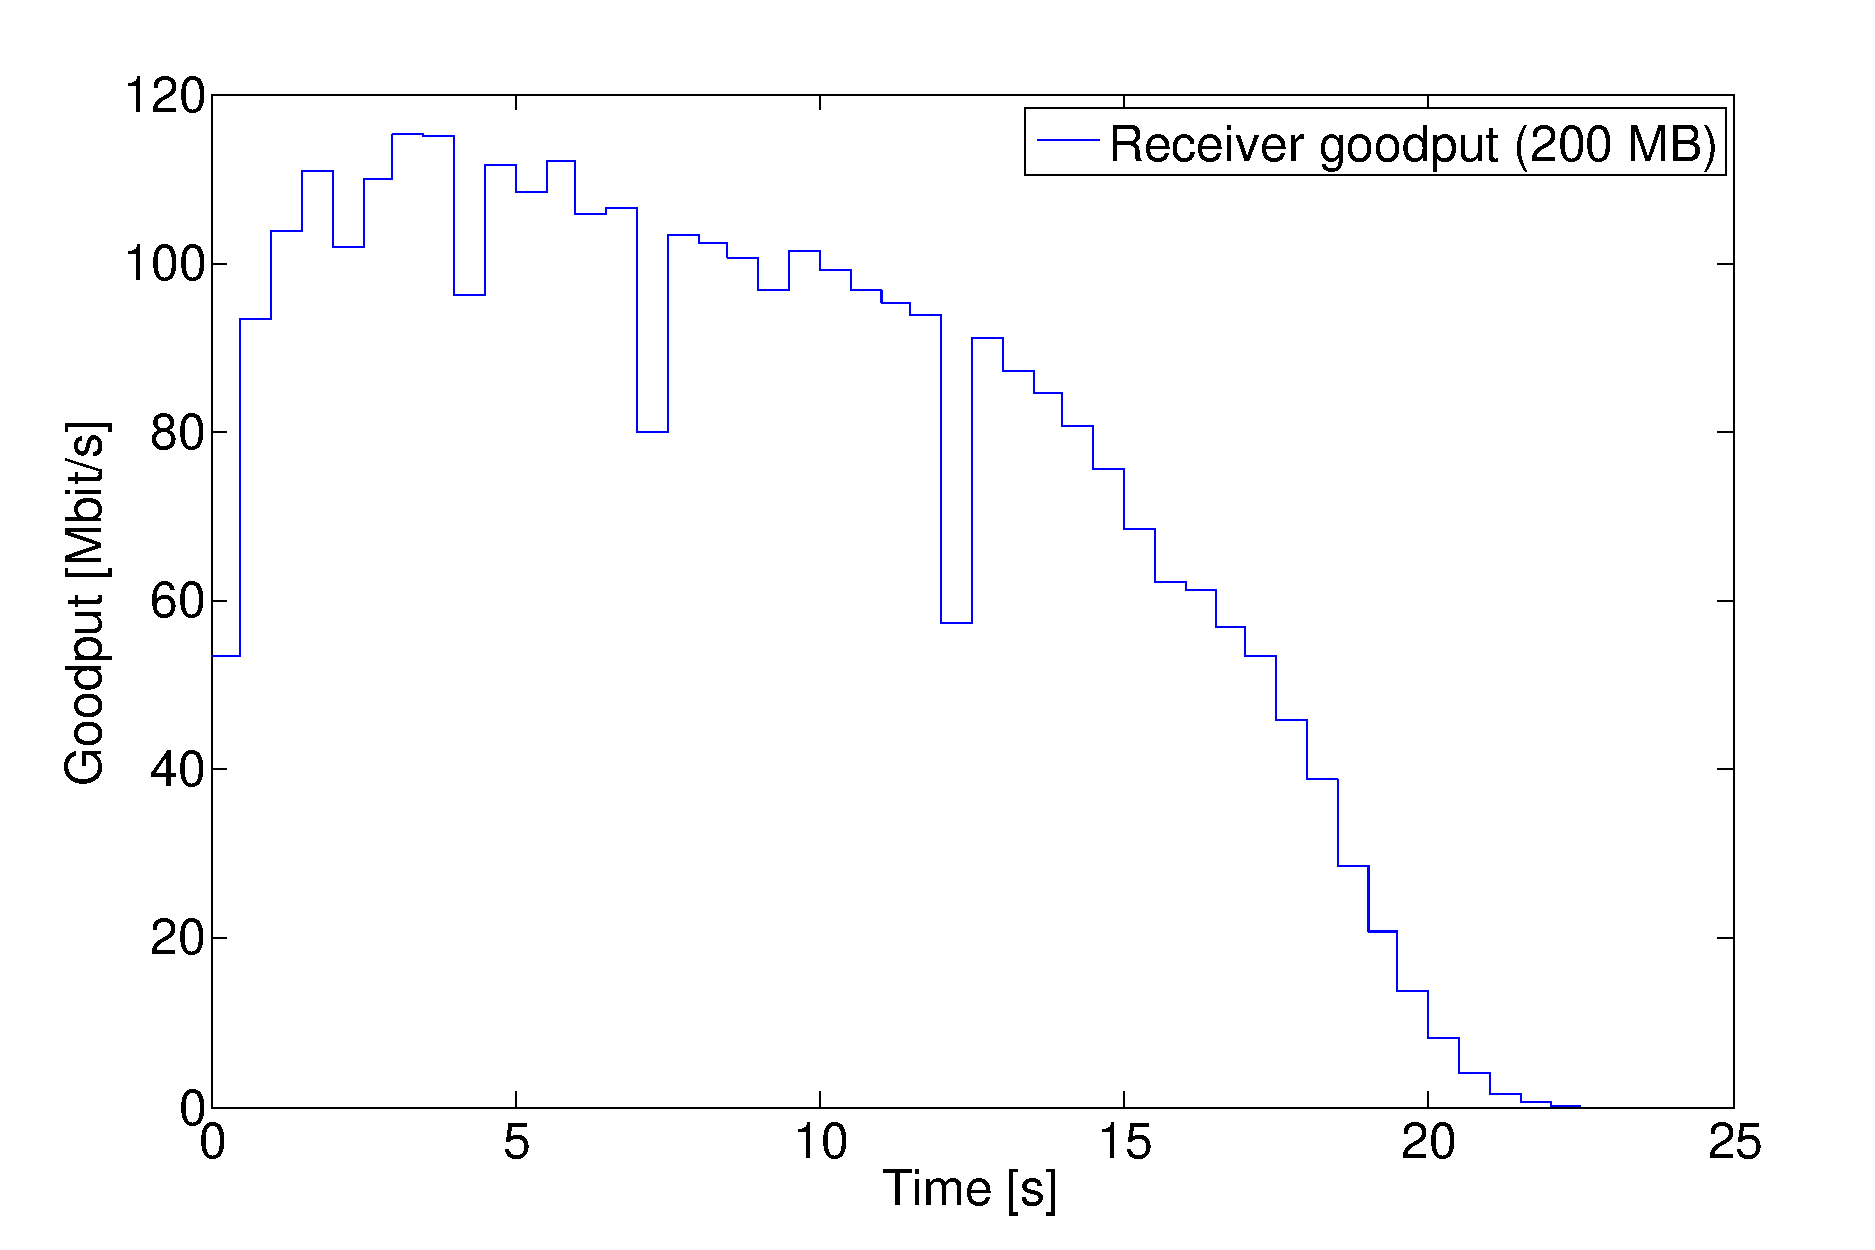
\includegraphics[width = 0.95\columnwidth, keepaspectratio]{tex/images/goodput_c2_200.pdf}
  \caption{Goodput at the receiver, file size 200 MB}
  \label{fig:goodput_200}
\end{figure}

\begin{figure}[h]
  \centering
  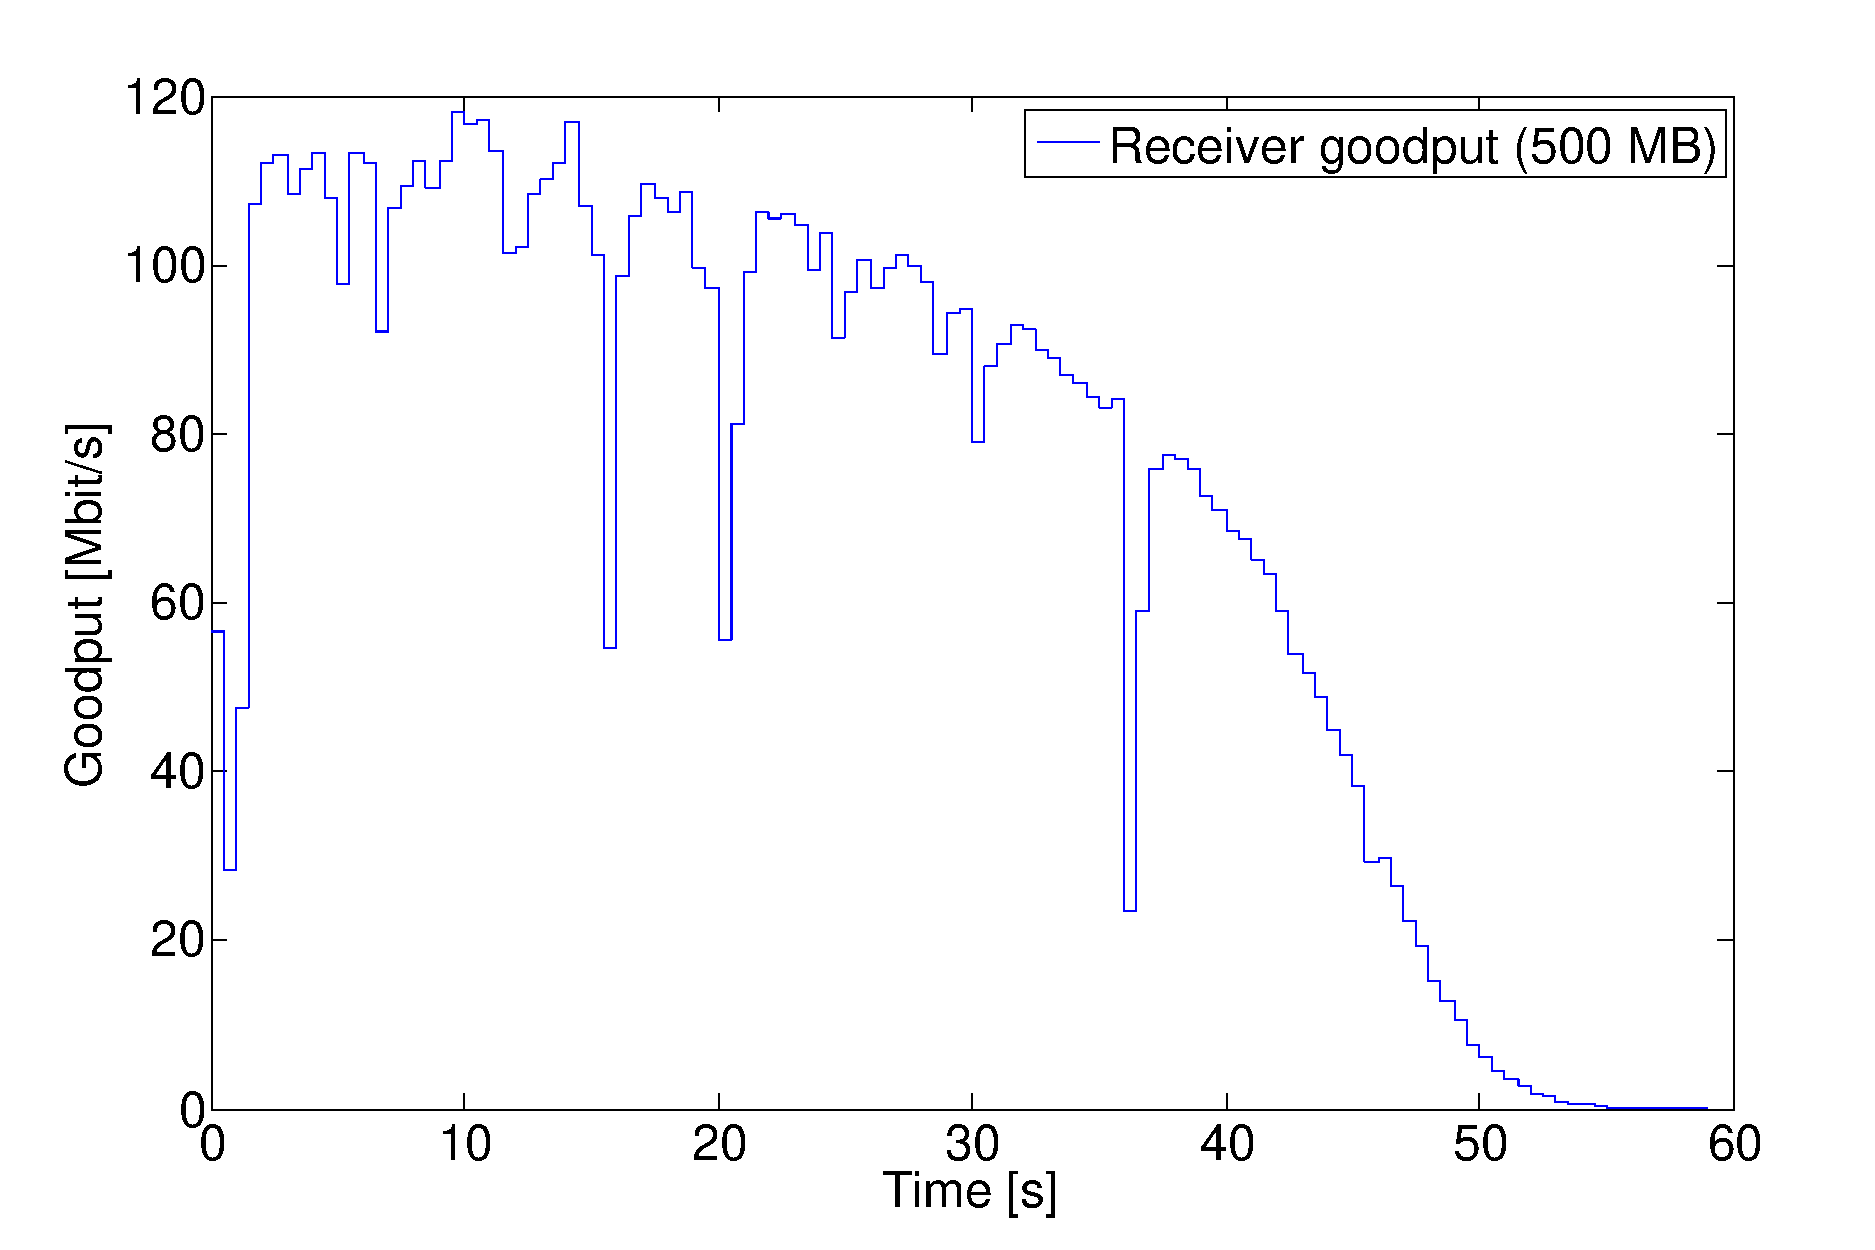
\includegraphics[width = 0.95\columnwidth, keepaspectratio]{tex/images/goodput_c1_500.pdf}
  \caption{Goodput at the receiver, file size 500 MB}
  \label{fig:goodput_500}
\end{figure}

\section{Concusions}
The HIPSTER protocol was designed in order to work upon networks with high rtt and high packet loss. Given the model of HIPSTER sender, receiver and TC, we developed a theoretical analysis in order to tune packet length. The implementation of the TC was tested and performed as expected. Finally, tests with files of different sizes showed that the protocol can reach high goodput and low transfer time.
\end{document}
